\chapter{Implementation}

\section{Libraries Used}
We chose Python as our primary language due to its fantastic machine learning support. PyTorch libraries provided excellent API for working with neural nets. The code involves 2 parts. One is the client(agent that is updating its neural net) and other is the environment that client is interacting with. Here the environment encapsulates the simspark server which actually executes actions and returns new state for the agent and runs the whole simulation. Many minor techniques of getting right acceleration values and checking if robot has fallen were obtained from repository of UT Austin Villa's code \cite{utaustin}. 

\section{Server Client Communication} 
Python Simspark agent \cite{pysimspark} was used to communicate with the simspark server. All communication between python-agent and simspark server was relayed through Environment class. We designed its interface similar to python open AI Gym environments. So we abstracted our reward calculation and implementation of features so that the agent could get the next state, reward and boolean flag for termination of episode from  a \texttt{step(action)} function. This takes action as input and gives the above mentioned outputs after performing one step in simulation. This is equivalent to performing a transition in the MDP \cite{Sutton:1998:IRL:551283} for this problem. After every episode, we reset the agent connection to start over. 
\\\\
We faced a lot of problems with this server environment. Since simspark server development is still under progress, it crashes if multiple connections are made and therefore, we have coded a robust environment handling all server side errors and subtly making A3C agent discard the given episode and restart whenever connection between server and client fails abruptly. Another bug in the server was the fact that instead of providing with the next state it gave the current state as the output at every time step. To handle this, we introduced a dummy 0 action between every two consecutive actions sent by the agent. This was meant to do nothing but get next state for the current action. Another issue with this server was the initial position of robot. Instead of being in rest pose on ground, the server initialized the agent in a free fall state. The agent landed on the ground and stabilized in about 1.2 seconds. Such errors took a lot of time to debug due to lack of proper documentation for simspark. Moreover, corrupting the input data this could have been the reason for our initial failures. 

\section{Getting rewards and next state}
Server provided most of the information to generate rewards and next state. The essentials things we received were orientations of 22 joints, our local position, accelerometer and gyrometer values. The rest of the state variables were calculated in the Environment class and abstracted out to the client.

\begin{figure}
\centering
  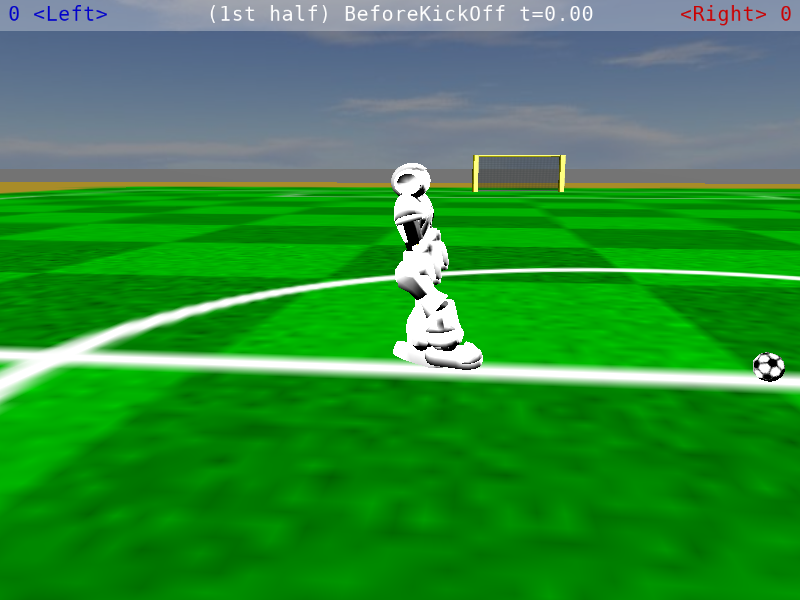
\includegraphics[width=0.5\linewidth, height=6cm,keepaspectratio]{images/monitor.png}
  \caption{Visualization of learning of robot using A3C on a standard Simspark Monitor}
  \label{fig:simulator}
\end{figure}

\section{Initial Pose and Rendering}
For retargeted motion, we had to use almost 50-100 frames to get to the initial pose of the motion via smooth transitions. This was ensured by getting one motion clip pose ahead of time and calculating the difference in orientations and then gradually decreasing this difference.
To visualize the progress while training the agent, we used the default standard monitor from simspark. The rendering part of the story was decoupled from the actual learning in the sense that one could visualize the agent only when required and not all the time while learning.

\section{Training A3C Agent}
The A3C \cite{pytorchaaac} was trained asynchronously with 4-5 different local threads learning the weights using the different instances of same environment independently. These threads periodically synchronized their updates to a global neural net. The weights were updated after each episode using a fixed learning rate.  

